% Created 2017-04-12 Wed 17:28
% Intended LaTeX compiler: pdflatex
\documentclass[a4paper,11pt]{article}
\usepackage[utf8]{inputenc}
\usepackage[T1]{fontenc}
\usepackage{graphicx}
\usepackage{grffile}
\usepackage{longtable}
\usepackage{wrapfig}
\usepackage{rotating}
\usepackage[normalem]{ulem}
\usepackage{amsmath}
\usepackage{textcomp}
\usepackage{amssymb}
\usepackage{capt-of}
\usepackage{hyperref}
\usepackage[margin=1.2in]{geometry}
\usepackage{setspace}
\onehalfspacing
\usepackage{parskip}
\setcounter{secnumdepth}{2}
\author{Zheng Tian}
\date{}
\title{An Introduction to Git and GitHub}
\hypersetup{
 pdfauthor={Zheng Tian},
 pdftitle={An Introduction to Git and GitHub},
 pdfkeywords={},
 pdfsubject={},
 pdfcreator={Emacs 25.1.1 (Org mode 9.0.3)},
 pdflang={English}}
\begin{document}

\maketitle


\section{What are Git and GitHub?}
\label{sec:orgf3949f2}

\subsection{What is Git?}
\label{sec:orgf22681d}

\begin{itemize}
\item Git is a version control system (VCS) that records changes to a file
or set of files over time so that you can recall specific versions
later.

\item Using Git to manage versions means that if you screw things up or
lose files, you can easily recover.
\end{itemize}

\subsection{How does Git work?}
\label{sec:orgd5f4b4c}

\begin{itemize}
\item Git takes a snapshot of a whole project whenever you make a commit
to the changes.
\end{itemize}
\begin{figure}[htbp]
\centering
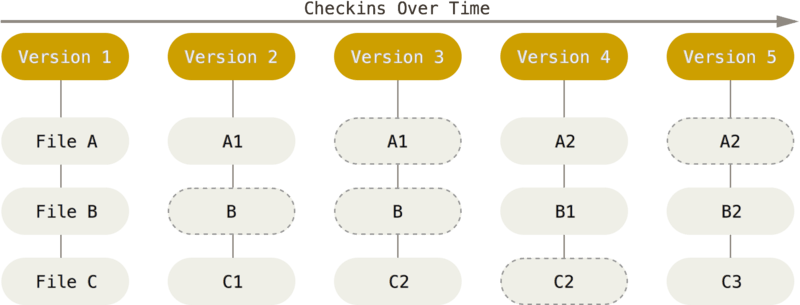
\includegraphics[width=.9\linewidth]{img/snapshots.png}
\caption{\label{fig:org2bd9b65}
Storing data as snapshots of the project over time}
\end{figure}

\subsection{The basic workflow of Git goes like this}
\label{sec:orge82cbb1}

\begin{enumerate}
\item You modify files in your working tree.
\item You stage the files, adding snapshots of them to your staging area.
\item You do a commit, which takes the files as they are in the staging
area and stores that snapshot permanently to your Git directory.
\end{enumerate}

\begin{figure}[htbp]
\centering
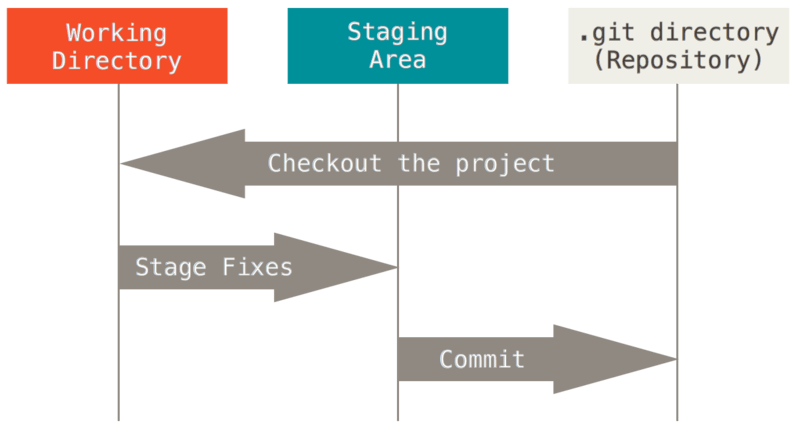
\includegraphics[width=.9\linewidth]{img/threestages.png}
\caption{\label{fig:org0db337a}
Working tree, staging area, and Git directory}
\end{figure}

\subsection{What is GitHub?}
\label{sec:orgb2dfedb}

\begin{itemize}
\item GitHub is the single largest host for Git repositories, and is the
central point of collaboration for millions of developers and
projects.

\item Visit \url{https://github.com/} and sign up a free account right now!
\end{itemize}


\section{Get Started}
\label{sec:org42e11c0}

\subsection{Install Git and GitHub Desktop}
\label{sec:org059b3f1}

\subsubsection*{Download and install Git}
\label{sec:orgf6fe525}

You can download the installers of Git for Windows, MacOS, and Linux at
\url{https://git-scm.com/downloads}.

\subsubsection*{Download and install GitHub Desktop}
\label{sec:org6fd8b6a}

\begin{itemize}
\item GitHub Desktop is a GUI for Git and integrate your repositories on
GitHub with local counterparts.
\item Download the installer of GitHub Desktop at
\url{https://desktop.github.com/}.
\end{itemize}

\subsection{Configure Git}
\label{sec:org46d8df8}

Next, follow the steps of configuration at
\url{https://help.github.com/articles/set-up-git/}.

\begin{enumerate}
\item Open a \textbf{terminal}.

\begin{itemize}
\item In MacOS, search \texttt{terminal} in Spotlight Search.
\item In Windows, open \texttt{Git Shell} that is installed with GitHub
Desktop.
\end{itemize}

\item Configure user name and user email. It is wise to use the same user
name and email when you sign up with GitHub.

\begin{verbatim}
$ git config --global user.name "YOUR NAME"
$ git config --global user.email "EMAIL ADDRESS"
\end{verbatim}

\item Setup a default editor. GitHub recommend using Atom.

\begin{itemize}
\item Download Atom at \url{https://atom.io/}.
\item Configure Atom to be the default editor of Git, as instructed at
\url{https://help.github.com/articles/associating-text-editors-with-git/}
In MacOS,
\begin{verbatim}
$ git config --global core.editor "atom --wait"
\end{verbatim}
In Windows
\begin{verbatim}
$ git config --global core.editor "C:/Users/USERNAME/AppData/Local/atom/app-VERSION/atom.exe"
\end{verbatim}
\end{itemize}

\item Authenticating Git with GitHub

\begin{itemize}
\item In MacOS. Install \texttt{osxkeychain helper} in by entering the
following command.
\begin{verbatim}
$ git credential-osxkeychain
\end{verbatim}
If \texttt{osxkeychain helper} has already been installed, nothing
happens. If not, your computer will prompt you to download it as
a part of the Xcode Command Line Tools.

\item In Windows. Open GitHub Desktop. If it is your first time opening it, a
window will pop up asking for your GitHub account.
\end{itemize}
\end{enumerate}

\subsection{Book: \emph{Pro Git}}
\label{sec:org4960d6f}

\begin{itemize}
\item Git is fully documented in this book,
\url{https://git-scm.com/book/en/v2}.
\end{itemize}


\section{{\bfseries\sffamily TODO} Git Basics [1/4]}
\label{sec:org71acf4f}

This section introduces the very basic commands of Git.

\subsection{{\bfseries\sffamily DONE} Create a Git repository}
\label{sec:orgb9aef2a}
A Git repository is simply a folder containing the files pertaining to
a project that you want to have versions controlled. Within the
folder, there is a sub-folder, usually invisible, called. \texttt{.git},
where all data regarding each different version are stored.

\subsubsection*{Create a Git repository in a computer}
\label{sec:orgd2e355b}

Let us first create a git repository in our computer. We do the
following things
\begin{itemize}
\item Create a new folder, called \texttt{git\_test}
\item Go to this folder
\item Make it a git repository.
\end{itemize}

\begin{verbatim}
$ mkdir git_test
$ cd git_test
$ git init
$ git status
\end{verbatim}

We use \texttt{git status} to check the status of the repository.

\subsubsection*{Create a Git repository in GitHub}
\label{sec:org5420443}

At \url{https:github.com}, click \textbf{New Repository} and follow the instruction
to create a new repository, names \texttt{github\_test}. This repository is
now at GitHub not in your computer. To make it in your computer, the
quickest way is to press the button of \textbf{Set up in Desktop}, which will
call GitHub Desktop and set up the repository in your computer.

Another way is the \texttt{HTTPS} of the repository and type the following
command, assuming that you are under a folder in which you want this new
repository to be downloaded.
\begin{verbatim}
$ git clone https://github.com/zngtian/github_test.git
$ git status
\end{verbatim}


\subsection{{\bfseries\sffamily TODO} Make a change and commit it}
\label{sec:orgf8d3668}

\subsubsection*{A life-cycle of a file in a git repository}
\label{sec:org130743d}

\begin{figure}[htbp]
\centering
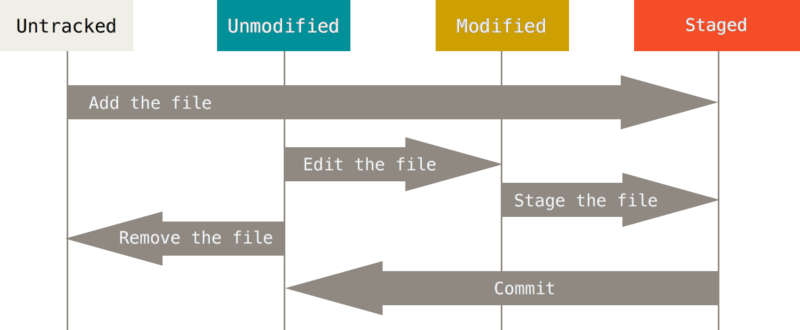
\includegraphics[width=0.8\textwidth]{img/lifecycle.png}
\caption{\label{fig:orgb95c3c7}
The lifecycle of the status of your files}
\end{figure}

Figure \ref{fig:orgb95c3c7}  displays a life cycle of a file in a git
repository.
\begin{itemize}
\item When a file is first created, its status in git is \textbf{untracked}. For
example, we create a new file \texttt{README.md}.
\item We want git to know that we have added a new file. With git, we need
to \textbf{stage} the file.
\item After we have made all changes regarding the new file, we need to
tell git that all changes are done. With git, we need to \textbf{commit}
the file.
\item After committing, if we make any change, we need to repeat staging
and committing.
\end{itemize}

All these things are implemented with the following command.
\begin{verbatim}
$ touch README.md
$ git add README.md
$ git commit -m "add a README.md file"
\end{verbatim}


\subsection{{\bfseries\sffamily TODO} What if I change my mind?}
\label{sec:org50824d4}



\subsection{{\bfseries\sffamily TODO} Make a new branch}
\label{sec:org22d3bb1}



\section{{\bfseries\sffamily TODO} A Workflow of Group Working}
\label{sec:orgc5355a5}
\end{document}